\documentclass{article}
\usepackage[utf8]{inputenc}
\usepackage{float}
\usepackage{color}
\usepackage{caption}
\usepackage{mwe}
\usepackage{relsize}

\title{SPL Test Report}
\date{September 2021}

\begin{document}

\maketitle

\section*{Introduction}

For task 3 we were asked to implement variability using a preprocessor. Our implementation uses Antenna. The following sections present the test report with several variants.

\section*{Variant 1}

In the first variant we use the configuration as given in figure \ref{fig:var1_config}. It has a command line interface with only logging enabled. The output can be viewed in figure \ref{fig:var1}. The top shows the server running while it prints some log information. Below that two clients are running. These clients have already connected without authentication and are messaging each other.

\begin{figure}[!htbp]
    \centering
    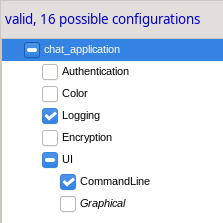
\includegraphics[width=0.5\textwidth]{figures/variant1_config.png}
    \caption{Variant 1 configuration}
    \label{fig:var1_config}
\end{figure}

\begin{figure}[!htbp]
    \centering
    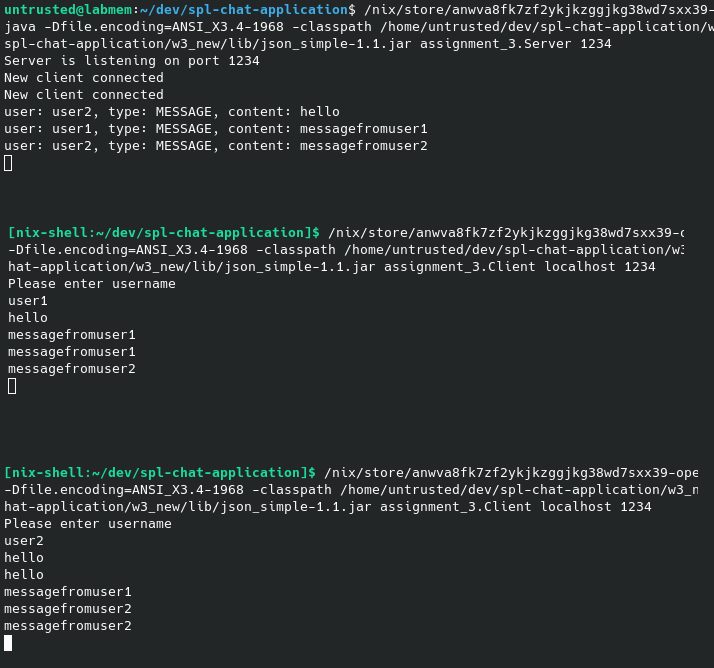
\includegraphics[width=1.0\textwidth]{figures/variant1.png}
    \caption{Variant 1 output showing a command line interface with logging}
    \label{fig:var1}
\end{figure}

\section*{Variant 2}

In the second variant we use the configuration as given in figure \ref{fig:var2_config}. It has a GUI with authentication enabled. The output can be viewed in figure \ref{fig:var2}. The top shows the server running without printing log information. Below that two GUI clients are running. These clients have authenticated with a username and password and are messaging each other.

\begin{figure}[!htbp]
    \centering
    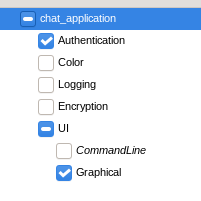
\includegraphics[width=0.5\textwidth]{figures/variant2_config.png}
    \caption{Variant 2 configuration}
    \label{fig:var2_config}
\end{figure}

\begin{figure}[!htbp]
    \centering
    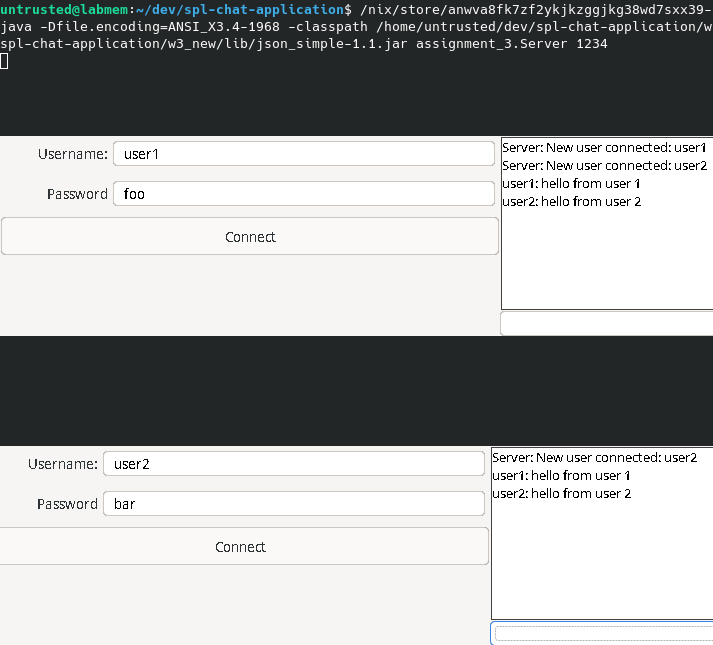
\includegraphics[width=1.0\textwidth]{figures/variant2.png}
    \caption{Variant 2 output showing a GUI with authentication}
    \label{fig:var2}
\end{figure}

\section*{Variant 3}

In the third variant we use the configuration as given in figure \ref{fig:var3_config}. It has a GUI with colors and encryption. The output can be viewed in figure \ref{fig:var3}. The top shows the server running without printing log information. Below that two GUI clients are running. The clients have not authenticated with a password. The text color can be selected by each client.

\begin{figure}[!htbp]
    \centering
    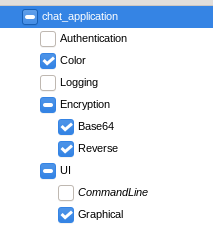
\includegraphics[width=0.5\textwidth]{figures/variant3_config.png}
    \caption{Variant 3 configuration}
    \label{fig:var3_config}
\end{figure}

\begin{figure}[!htbp]
    \centering
    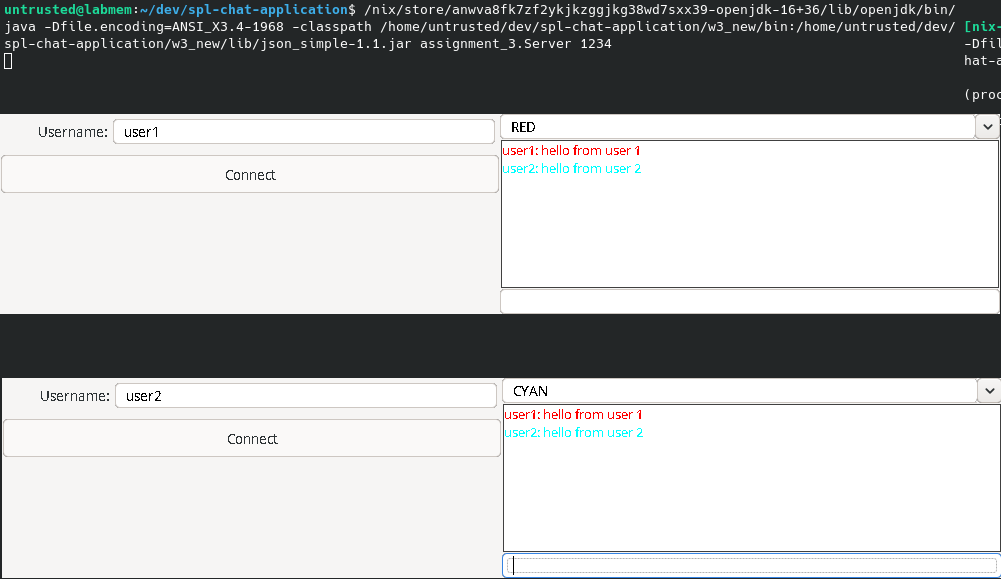
\includegraphics[width=1.0\textwidth]{figures/variant3.png}
    \caption{Variant 3 output showing a GUI with encryption and colored text}
    \label{fig:var3}
\end{figure}

\end{document}
